\documentclass[12pt,a4paper]{book}

\usepackage[margin=2.5cm]{geometry}
\usepackage[T1]{fontenc}
\usepackage[utf8]{inputenc}
\usepackage{lmodern}
\usepackage{hyperref}
\usepackage{xcolor}
\usepackage{listings}
\usepackage{enumitem}
\usepackage{graphicx}
\usepackage{csquotes}
\usepackage{amssymb}


\hypersetup{
  colorlinks=true,
  linkcolor=blue,
  urlcolor=blue,
  citecolor=blue
}

\lstdefinestyle{bashstyle}{
  basicstyle=\ttfamily\small,
  breaklines=true,
  frame=single
}

\title{Running Bitcoin Core or Bitcoin Knots\\
\large A Practical Guide to Installing a Full Node\\
and Backing Up Your Wallet on Paper, Metal, and More}
\author{(Your Name Here)}
\date{\today}

\begin{document}
\begin{titlepage}
    \centering
    \vspace*{3cm}

    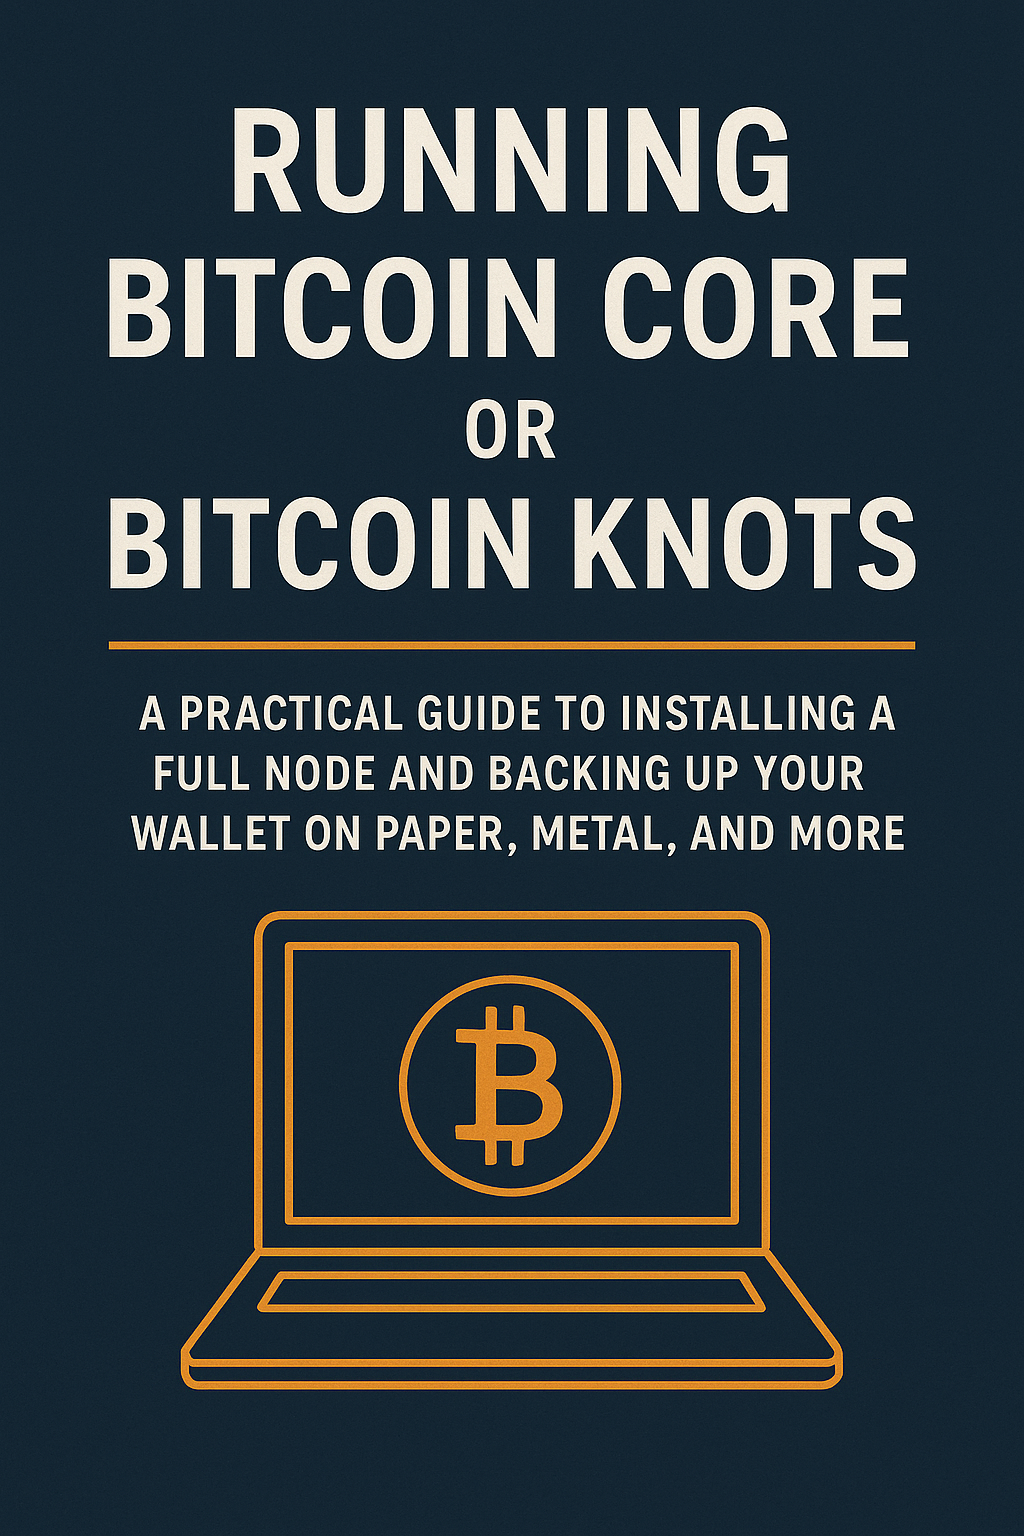
\includegraphics[width=0.85\textwidth]{bitcoin_node_cover.png}

    \vfill
\end{titlepage}


\maketitle
\tableofcontents

\chapter*{Preface}

This book is a practical guide for individuals who want to:

\begin{itemize}
  \item Install and run a Bitcoin full node using Bitcoin Core or Bitcoin Knots.
  \item Create a wallet for personal funds.
  \item Back up that wallet safely using a combination of digital, paper, and metal backups.
\end{itemize}

It is written for non-experts who are comfortable following step-by-step instructions and copying commands, but it includes enough detail to be useful for more technical readers as well.

The focus is on:
\begin{itemize}
  \item \textbf{Security:} Not losing coins and not having them stolen.
  \item \textbf{Simplicity:} A clear, repeatable process suited to personal funds.
  \item \textbf{Self-sovereignty:} You verify Bitcoin yourself, and you control your keys.
\end{itemize}

This book does not cover trading, speculative strategies, or custodial services. It is about self-custody over your own full node.

\chapter{Fundamentals}

\section{What Is a Bitcoin Full Node?}

A Bitcoin full node is software that:
\begin{itemize}
  \item Downloads and verifies every block and transaction according to the Bitcoin protocol rules.
  \item Relays valid transactions and blocks to other nodes.
  \item Provides a local view of the network that you can trust without asking anyone else.
\end{itemize}

Running your own full node gives you:
\begin{itemize}
  \item \textbf{Independent verification:} You do not trust an exchange or wallet app to tell you what is valid.
  \item \textbf{Privacy:} When you query your own node, you do not leak wallet information to a third-party server.
  \item \textbf{Control:} You can enforce your own policy (for example, which features or rules you accept).
\end{itemize}

\section{Bitcoin Core vs. Bitcoin Knots}

\textbf{Bitcoin Core} is the reference implementation of the Bitcoin protocol. It is the most widely used full node software.

\textbf{Bitcoin Knots} is a derivative of Bitcoin Core maintained by a different developer. It:
\begin{itemize}
  \item Uses Bitcoin Core as a base.
  \item Adds extra features and options aimed at power users.
  \item Is usually compatible with the same blockchain rules, but may have different policy defaults.
\end{itemize}

For most beginners:
\begin{itemize}
  \item Bitcoin Core is a perfectly safe and well-supported choice.
  \item Bitcoin Knots is suitable if you are comfortable with more advanced options and want additional features.
\end{itemize}

\section{Keys, Wallets, and Backups}

To control Bitcoin, you need \textbf{private keys}. A \emph{wallet} is software and/or a file that:
\begin{itemize}
  \item Stores your private keys.
  \item Derives addresses where you can receive Bitcoin.
  \item Signs transactions to spend those coins.
\end{itemize}

In Bitcoin Core / Knots:
\begin{itemize}
  \item A wallet is stored as a file (traditionally \texttt{wallet.dat}) inside the data directory.
  \item Modern wallets are HD (hierarchical deterministic), deriving many keys from a single root seed.
  \item You can encrypt the wallet with a passphrase.
\end{itemize}

\textbf{Backups} are critical. If you lose your keys and have no backup, \emph{your coins are lost forever}. There is no password reset, no support desk that can recover them.

We will focus on:
\begin{itemize}
  \item Digital backups (copies of the encrypted wallet file).
  \item Paper backups (writing recovery material on paper).
  \item Metal backups (engraving or stamping key material in metal).
\end{itemize}

\section{Threat Model for Personal Funds}

Before deciding how to back up, think about your threats:

\begin{itemize}
  \item \textbf{Accidental loss:} Hard drive failure, device lost or destroyed, you forget where you stored it.
  \item \textbf{Theft:} Someone physically steals your backup or compromises your computer.
  \item \textbf{Coercion:} Someone forces you to reveal a passphrase.
  \item \textbf{Natural disasters:} Fire, flood, or other events that can destroy paper and electronics.
\end{itemize}

We will aim for a practical balance:
\begin{itemize}
  \item For small to medium personal savings, one or two encrypted digital backups plus one physical backup (paper or metal) is usually enough.
  \item For life-changing money, more redundancy and better physical security are strongly recommended.
\end{itemize}

\chapter{Preparing Your System}

\section{Hardware Requirements}

A typical full node requires:

\begin{itemize}
  \item \textbf{Storage:} At least several hundred gigabytes of disk space for the blockchain (preferably SSD).
  \item \textbf{RAM:} 4~GB or more is recommended.
  \item \textbf{CPU:} Any modern 64-bit CPU is fine; initial sync is CPU and disk intensive.
  \item \textbf{Network:} A stable internet connection; several hundred gigabytes of bandwidth during initial sync.
\end{itemize}

\section{Operating System Considerations}

Bitcoin Core and Knots both support:

\begin{itemize}
  \item GNU/Linux distributions.
  \item Windows (64-bit).
  \item macOS (recent versions).
\end{itemize}

This book will show example commands mostly using:
\begin{itemize}
  \item Linux command line.
  \item Some general notes for Windows and macOS.
\end{itemize}

\section{Basic Security Hygiene}

Before dealing with money:

\begin{itemize}
  \item Keep your operating system up to date.
  \item Use full-disk encryption where possible.
  \item Use a unique, strong password for your computer.
  \item Avoid installing random software from untrusted sources.
  \item Consider having a dedicated machine (or at least a dedicated user account) for your node and wallet.
\end{itemize}

\chapter{Downloading and Verifying Bitcoin Core / Knots}

\section{Where to Download}

\textbf{Important:} Always download from official sources and verify signatures. Do not rely on search engine ads or random links.

At the time of writing, official project sites are:

\begin{itemize}
  \item Bitcoin Core: \url{https://bitcoincore.org/}
  \item Bitcoin Knots: \url{https://bitcoinknots.org/}
\end{itemize}

Navigate to the downloads section appropriate for your operating system.

\section{Verifying PGP Signatures (Linux Example)}

The Bitcoin Core / Knots releases are signed by developers using PGP. Verifying the signature helps ensure that:

\begin{itemize}
  \item The file was not tampered with in transit.
  \item You are not installing malware.
\end{itemize}

\subsection*{Step 1: Download the Binary and Signature}

For example (Linux, 64-bit, Bitcoin Core):

\begin{lstlisting}[style=bashstyle]
wget https://bitcoincore.org/bin/bitcoin-core-XX.Y.Z/bitcoin-XX.Y.Z-x86_64-linux-gnu.tar.gz
wget https://bitcoincore.org/bin/bitcoin-core-XX.Y.Z/SHA256SUMS.asc
\end{lstlisting}

Replace \texttt{XX.Y.Z} with the current version.

\subsection*{Step 2: Import the Release Signing Key}

On the official website, you will find a link to the release signing keys. Download and import it:

\begin{lstlisting}[style=bashstyle]
gpg --keyserver keyserver.ubuntu.com --recv-keys <KEYID>
\end{lstlisting}

Verify the fingerprint against the fingerprint listed on the official site.

\subsection*{Step 3: Verify the Signature and Checksums}

Check the signature:

\begin{lstlisting}[style=bashstyle]
gpg --verify SHA256SUMS.asc
\end{lstlisting}

Then verify checksums:

\begin{lstlisting}[style=bashstyle]
sha256sum bitcoin-XX.Y.Z-x86_64-linux-gnu.tar.gz
\end{lstlisting}

Ensure the hash matches the entry for your file in \texttt{SHA256SUMS.asc}.

\section{Windows and macOS Verification (High-Level)}

On Windows and macOS the idea is the same:

\begin{enumerate}
  \item Download the installer and the signature or checksums file from the official site.
  \item Install GnuPG (or use an existing PGP tool).
  \item Import the release signing key and verify the signature.
\end{enumerate}

If you do not feel comfortable with PGP yet:

\begin{itemize}
  \item At a minimum, verify checksums from the official site.
  \item Learn PGP signature verification later as a security upgrade.
\end{itemize}

\chapter{Installing Bitcoin Core / Knots}

\section{Linux (Tarball Installation)}

After verifying:

\begin{lstlisting}[style=bashstyle]
tar -xzf bitcoin-XX.Y.Z-x86_64-linux-gnu.tar.gz
cd bitcoin-XX.Y.Z/bin
\end{lstlisting}

You can either:
\begin{itemize}
  \item Run binaries from this directory, or
  \item Copy them to a location like \texttt{/usr/local/bin}:
\end{itemize}

\begin{lstlisting}[style=bashstyle]
sudo install -m 0755 -o root -g root -t /usr/local/bin bitcoind bitcoin-cli bitcoin-qt
\end{lstlisting}

\section{Windows Installation}

\begin{enumerate}
  \item Download the Windows installer (\texttt{.exe}) from the official site.
  \item Double-click the installer and follow the prompts.
  \item Choose a data directory (you can accept the default or select a larger drive).
\end{enumerate}

After installation:
\begin{itemize}
  \item You can run Bitcoin Core (or Knots) from the Start menu.
  \item The initial setup wizard will ask about pruning and data directory.
\end{itemize}

\section{macOS Installation}

\begin{enumerate}
  \item Download the \texttt{.dmg} file.
  \item Open it and drag the Bitcoin Core (or Knots) app into \texttt{/Applications}.
  \item Launch the application; on first run, macOS may warn you about unsigned apps --- follow the official instructions for bypassing this if needed.
\end{enumerate}

\section{Pruned Node vs. Full Archive Node}

On first launch, you will be asked if you want a pruned node.

\begin{itemize}
  \item \textbf{Full node (non-pruned):} Keeps the entire blockchain history. Requires more disk space.
  \item \textbf{Pruned node:} Keeps only recent blocks and discards old ones after verifying them. Saves disk space.
\end{itemize}

For personal use:
\begin{itemize}
  \item A pruned node is usually fine and much easier on storage.
  \item Wallet functions work with both.
\end{itemize}

\chapter{Configuring and Running the Node}

\section{Data Directory and Configuration File}

The data directory stores:
\begin{itemize}
  \item Blockchain data.
  \item Wallet files.
  \item Logs.
  \item Configuration file (\texttt{bitcoin.conf} or \texttt{bitcoin-knots.conf}).
\end{itemize}

Typical default locations:

\begin{itemize}
  \item Linux: \texttt{\$HOME/.bitcoin}
  \item Windows: \texttt{\%APPDATA\%\\Bitcoin}
  \item macOS: \texttt{\$HOME/Library/Application Support/Bitcoin}
\end{itemize}

You can create or edit \texttt{bitcoin.conf} in that directory. Example:

\begin{lstlisting}[style=bashstyle]
# bitcoin.conf example
server=1
txindex=0
prune=550
rpcuser=youruser
rpcpassword=long_random_password_here
\end{lstlisting}

\section{Starting the Node}

On Linux:

\begin{lstlisting}[style=bashstyle]
bitcoind -daemon
\end{lstlisting}

On Windows/macOS you can run the GUI (Bitcoin Qt) or a background daemon depending on your preference.

\section{Monitoring Sync Progress}

Use the GUI or command line:

\begin{lstlisting}[style=bashstyle]
bitcoin-cli getblockchaininfo
\end{lstlisting}

Look at:

\begin{itemize}
  \item \texttt{blocks} vs \texttt{headers} (how far along you are).
  \item \texttt{verificationprogress} (0 to 1).
\end{itemize}

Initial sync can take many hours or days, depending on hardware and network.

\chapter{Creating a Wallet}

\section{Legacy vs. Modern (Descriptor) Wallets}

Modern Bitcoin Core uses descriptor wallets by default. This is good for:

\begin{itemize}
  \item Cleaner structure of keys and scripts.
  \item Better compatibility with multisig and advanced setups.
\end{itemize}

You can create wallets via GUI or CLI.

\section{Creating a Wallet (GUI)}

\begin{enumerate}
  \item Open Bitcoin Core (or Knots) GUI.
  \item Go to \textbf{File} $\rightarrow$ \textbf{Create Wallet}.
  \item Choose a wallet name (e.g., \enquote{PersonalSavings}).
  \item Ensure \enquote{Encrypt wallet} is checked.
  \item Confirm the creation and set a strong passphrase when prompted.
\end{enumerate}

\textbf{Passphrase rules:}
\begin{itemize}
  \item Make it long (at least 12--16 words or random characters).
  \item Do not reuse a password from any other site or service.
  \item Consider writing a hint for yourself (not the whole passphrase) in a separate place.
\end{itemize}

\section{Creating a Wallet (CLI)}

Example:

\begin{lstlisting}[style=bashstyle]
bitcoin-cli createwallet "PersonalSavings" true
\end{lstlisting}

The \texttt{true} parameter means: create an encrypted wallet. You will be prompted to set a passphrase or need to encrypt afterward, depending on version.

To encrypt an existing wallet:

\begin{lstlisting}[style=bashstyle]
bitcoin-cli encryptwallet -stdinwalletpassphrase
\end{lstlisting}

\section{Receiving a Test Transaction}

Before putting significant funds:

\begin{enumerate}
  \item Get a receiving address in the wallet (\textbf{Receive} tab in GUI or \texttt{getnewaddress} in CLI).
  \item Send a tiny amount of BTC from an exchange or another wallet.
  \item Wait for confirmations.
  \item Practice listing transactions with \texttt{listtransactions}.
\end{enumerate}

This ensures everything works and gives you a chance to practice backups with low risk.

\chapter{Backing Up the Wallet File}

\section{Understanding \texttt{wallet.dat}}

The \texttt{wallet.dat} file (or descriptor wallet files) contain:

\begin{itemize}
  \item Your private keys (encrypted if you set a passphrase).
  \item Metadata about transactions and addresses.
  \item For descriptor wallets, descriptors that define how keys and addresses are derived.
\end{itemize}

\textbf{If your wallet is encrypted and you have a copy of \texttt{wallet.dat}, you can restore access to your coins.}

\section{Back Up from the GUI}

\begin{enumerate}
  \item Open your wallet in the GUI.
  \item Go to \textbf{File} $\rightarrow$ \textbf{Backup Wallet}.
  \item Choose a location (USB stick, external drive).
  \item Save the backup file (you can rename it, e.g. \texttt{personal\_wallet\_backup.dat}).
\end{enumerate}

Repeat this step for:
\begin{itemize}
  \item At least one offline USB drive stored safely.
  \item Optionally, a second backup in another location.
\end{itemize}

\section{Back Up from the CLI}

Use:

\begin{lstlisting}[style=bashstyle]
bitcoin-cli backupwallet "/path/to/backup/wallet-backup.dat"
\end{lstlisting}

Make sure:
\begin{itemize}
  \item The directory exists.
  \item The backup destination is on a drive you can physically remove and store.
\end{itemize}

\section{Storing Digital Backups Safely}

\begin{itemize}
  \item Use \textbf{encrypted} external drives when possible.
  \item Store backups in at least two different physical locations (e.g., home and a trusted relative's place, or a safe deposit box).
  \item Label backups clearly but not attractively (avoid writing \enquote{Bitcoin riches} on the USB stick).
  \item Periodically plug the backup into a computer to ensure it still reads (without exposing it to untrusted machines).
\end{itemize}

\chapter{Paper and Metal Backups}

\section{Important Warning About Text Backups}

Any backup that exposes raw private keys or wallet seed material in human-readable form (paper, metal, photos) can be:
\begin{itemize}
  \item Stolen by anyone who sees or photographs it.
  \item Lost if you misplace the paper/metal.
  \item Coercively extracted.
\end{itemize}

\textbf{Never store unencrypted digital copies (e.g., photos) of your seed or private keys in the cloud, email, or on your phone.}

\section{Approach 1: Seed Phrase from an External Wallet}

Bitcoin Core itself does not present a simple BIP39 seed phrase in the GUI. One common pattern is:
\begin{itemize}
  \item Use a hardware wallet or BIP39-compatible software wallet to generate a seed phrase.
  \item Connect that wallet to your Bitcoin Core / Knots node for transaction broadcasting and verification.
  \item Write the seed phrase on paper or metal and store it securely.
\end{itemize}

This combines:
\begin{itemize}
  \item Full-node verification.
  \item Simple human-readable backup (seed phrase).
\end{itemize}

\section{Approach 2: Descriptor and Key Export (Advanced)}

For advanced users, Bitcoin Core supports exporting descriptors or keys. This can be used to create a paper or metal backup.

Examples (do not run blindly, understand the privacy implications):

\begin{lstlisting}[style=bashstyle]
bitcoin-cli getwalletdescriptorinfo "$(bitcoin-cli listdescriptors false)"
\end{lstlisting}

or

\begin{lstlisting}[style=bashstyle]
bitcoin-cli dumpwallet "/path/to/dump.txt"
\end{lstlisting}

\textbf{Warning:} \texttt{dumpwallet} exposes all private keys in plaintext. Treat the resulting file as extremely sensitive and delete it securely once you have transferred the information you need.

If you choose to go this route:
\begin{itemize}
  \item Use an offline machine if possible.
  \item Never leave the dump file on an internet-connected device longer than necessary.
  \item Carefully transcribe required keys or descriptors onto paper or metal.
\end{itemize}

\section{Making a Paper Backup}

For a seed phrase (from a hardware or BIP39 wallet):

\begin{enumerate}
  \item Write each word clearly in order.
  \item Use a pen that does not smudge easily.
  \item Consider writing a second copy and storing it in a different location.
  \item Optionally add a checksum or small mark so you can detect if pages are missing.
\end{enumerate}

For descriptors or keys (advanced):

\begin{itemize}
  \item Print or write them clearly.
  \item Prefer short, structured data (like descriptors) over long lists of keys.
\end{itemize}

\section{Making a Metal Backup}

Metal backups are designed to survive:

\begin{itemize}
  \item Fire.
  \item Water damage.
  \item Physical degradation that would destroy paper.
\end{itemize}

Typical methods:

\begin{itemize}
  \item Letter punch set and steel plates.
  \item Commercial metal backup kits that support placing letters for BIP39 words.
\end{itemize}

Guidelines:

\begin{itemize}
  \item Work in a private area away from cameras.
  \item Double-check each word or character before finalizing.
  \item Store metal backups in a safe, lockbox, or other secure location.
\end{itemize}

\chapter{Restoring From Backups}

\section{Restoring from \texttt{wallet.dat}}

Scenario: Your computer dies, but you still have your encrypted wallet backup.

\begin{enumerate}
  \item Install Bitcoin Core or Knots on a new machine.
  \item Let it sync (or at least sync up to a point where your wallet's transactions can be seen).
  \item Close the node software completely.
  \item Copy your backup file into the data directory's \texttt{wallets} folder (or main directory for older setups).
  \item Start the node.
  \item In the GUI, go to \textbf{File} $\rightarrow$ \textbf{Open Wallet} and select your restored wallet.
  \item Unlock the wallet with your passphrase.
\end{enumerate}

\section{Restoring from a Seed Phrase (External Wallet)}

If you used a BIP39-compatible hardware or software wallet:

\begin{enumerate}
  \item On a new device, install the same wallet software (or another compatible wallet).
  \item Choose \enquote{Restore from seed phrase}.
  \item Enter your 12/24 words in the correct order.
  \item The wallet will recreate keys and addresses.
  \item Connect this wallet again to your Bitcoin Core / Knots node if desired.
\end{enumerate}

\section{Testing Your Backups}

You should periodically test backup procedures with low amounts:

\begin{enumerate}
  \item Create a small \enquote{test wallet}.
  \item Fund it with a tiny amount of BTC.
  \item Back it up using your chosen method.
  \item Wipe the wallet from your computer (or use a separate device).
  \item Restore from the backup and confirm you can access the coins.
\end{enumerate}

Do this before relying on any method for life-changing funds.

\chapter{Operational Best Practices}

\section{Separating Hot and Cold Funds}

Consider:

\begin{itemize}
  \item \textbf{Hot wallet:} Small amount for spending; may be on a device connected to the internet regularly.
  \item \textbf{Cold wallet:} Larger savings; keys never touch an internet-connected device (hardware wallet or offline setup).
\end{itemize}

\section{Passphrase Management}

\begin{itemize}
  \item Use a \textbf{password manager} for random, strong passwords for everything except the wallet itself.
  \item For wallet encryption, many prefer a passphrase they can remember (with written hints stored separately).
  \item Never reuse wallet passphrases on websites or other services.
\end{itemize}

\section{Privacy Considerations}

\begin{itemize}
  \item Running your own node improves privacy, but:
  \item Avoid reusing addresses.
  \item Be cautious about linking your identity to your addresses (for example by posting them publicly).
\end{itemize}

\section{Keeping Software Up to Date}

\begin{itemize}
  \item Update Bitcoin Core / Knots periodically.
  \item Before updating, verify signatures as you did initially.
  \item Always keep backups that were made \emph{before} the upgrade, in case a bug or migration issue occurs.
\end{itemize}

\chapter{Checklists}

\section{Initial Setup Checklist}

\begin{enumerate}
  \item Download Bitcoin Core or Knots from the official site.
  \item Verify PGP signatures and checksums.
  \item Install on your computer.
  \item Configure \texttt{bitcoin.conf} with your desired options (pruning, data directory).
  \item Start the node and wait for sync.
  \item Create an encrypted wallet with a strong passphrase.
  \item Make at least two digital backups of the wallet file on separate removable media.
\end{enumerate}

\section{Backup Checklist}

\begin{itemize}
  \item[\(\square\)] Wallet is encrypted with a strong, unique passphrase.
  \item[\(\square\)] At least one encrypted digital backup stored offline.
  \item[\(\square\)] Second encrypted digital backup stored in a different location.
  \item[\(\square\)] Optional: paper or metal backup of seed phrase (if using BIP39/hardware wallet).
  \item[\(\square\)] Tested restore procedure with small funds.
\end{itemize}

\section{Periodic Maintenance Checklist}

\begin{itemize}
  \item[\(\square\)] Check that node is syncing correctly.
  \item[\(\square\)] Confirm external backup drives still work.
  \item[\(\square\)] Review physical backup locations for signs of damage or risk.
  \item[\(\square\)] Update node software when new stable versions are released, after verification.
\end{itemize}

\chapter*{Conclusion}

Running your own Bitcoin full node and backing up your wallet properly is one of the most empowering things you can do in the digital age. It lets you:

\begin{itemize}
  \item Verify your own money.
  \item Control your own keys.
  \item Reduce reliance on trusted third parties.
\end{itemize}

With careful backups on digital media, paper, and metal, you can protect your savings against both accidents and attacks. Start with small amounts, practice the full cycle of backup and restore, and gradually grow your confidence and your self-sovereignty.

\end{document}
